\section{Software architecture views}
asdf
\subsection{Subsystem decomposition}
asdf
\subsection{Hardware/software mapping}
asdf
\subsection{Persistent data management}



The data management for our project envelops multiple things. We have a part where the data for the game is stored and the data we need for running the agent. The first part is done by Tygron. When a new project is created it is stored in the Tygron database to which the clients can connect via the Tygron server. Any changes made in a session are then updated to the database, which are visible to all the other clients. Figure \ref{fig:tygron1} shows the diagram of the Tygron Engine connected to the database and the GOAL agent.

\begin{figure}[h!]
  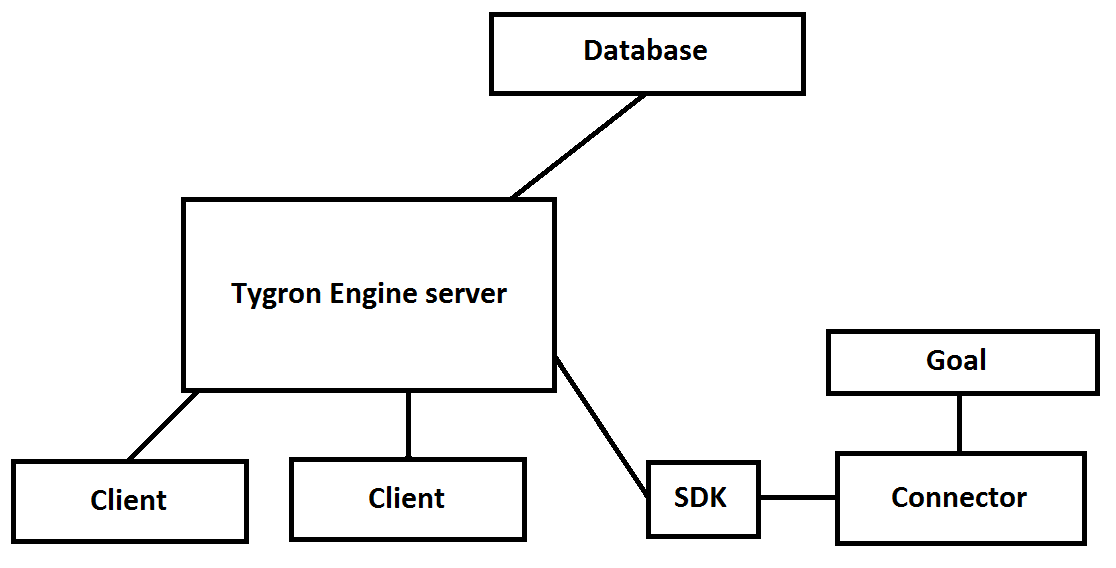
\includegraphics[width=\linewidth]{Tygrondatabase.png}
  \caption{Diagram of the Tygron Engine connected to the database and the GOAL agent.}
  \label{fig:tygron1}
\end{figure}

In GOAL the data the agent uses is stored in multiple databases. The agent has a knowledge base which is the same for every environment that he might find himself in. This data is simply stored as GOAL code in the agent his GOAL files. The rest of the data that the agent uses is dynamic and his state is updated constantly according to the situation that the agent is currently in. Our agent maintains two different databases of facts. One database called the goal base consists of things the agent wants to achieve. The other database is called the belief base and consists of facts that the agent believes are true (now).  Figure \ref{fig:agentstate1} shows how the databases of the agent are updated.

\begin{figure}[h!]
  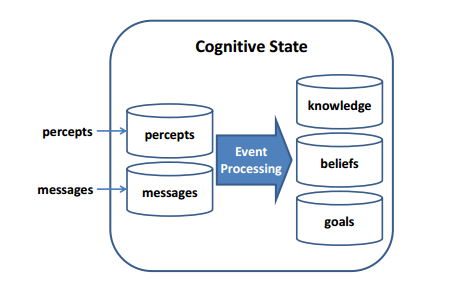
\includegraphics[width=\linewidth]{agentstate.png}
  \caption{Updating the agent's database.}
  \label{fig:agentstate1}
\end{figure}

\subsection{Concurrency}





